\begin{figure*}[htbp!]
	\begin{center}
	\resizebox{\textwidth}{!}{
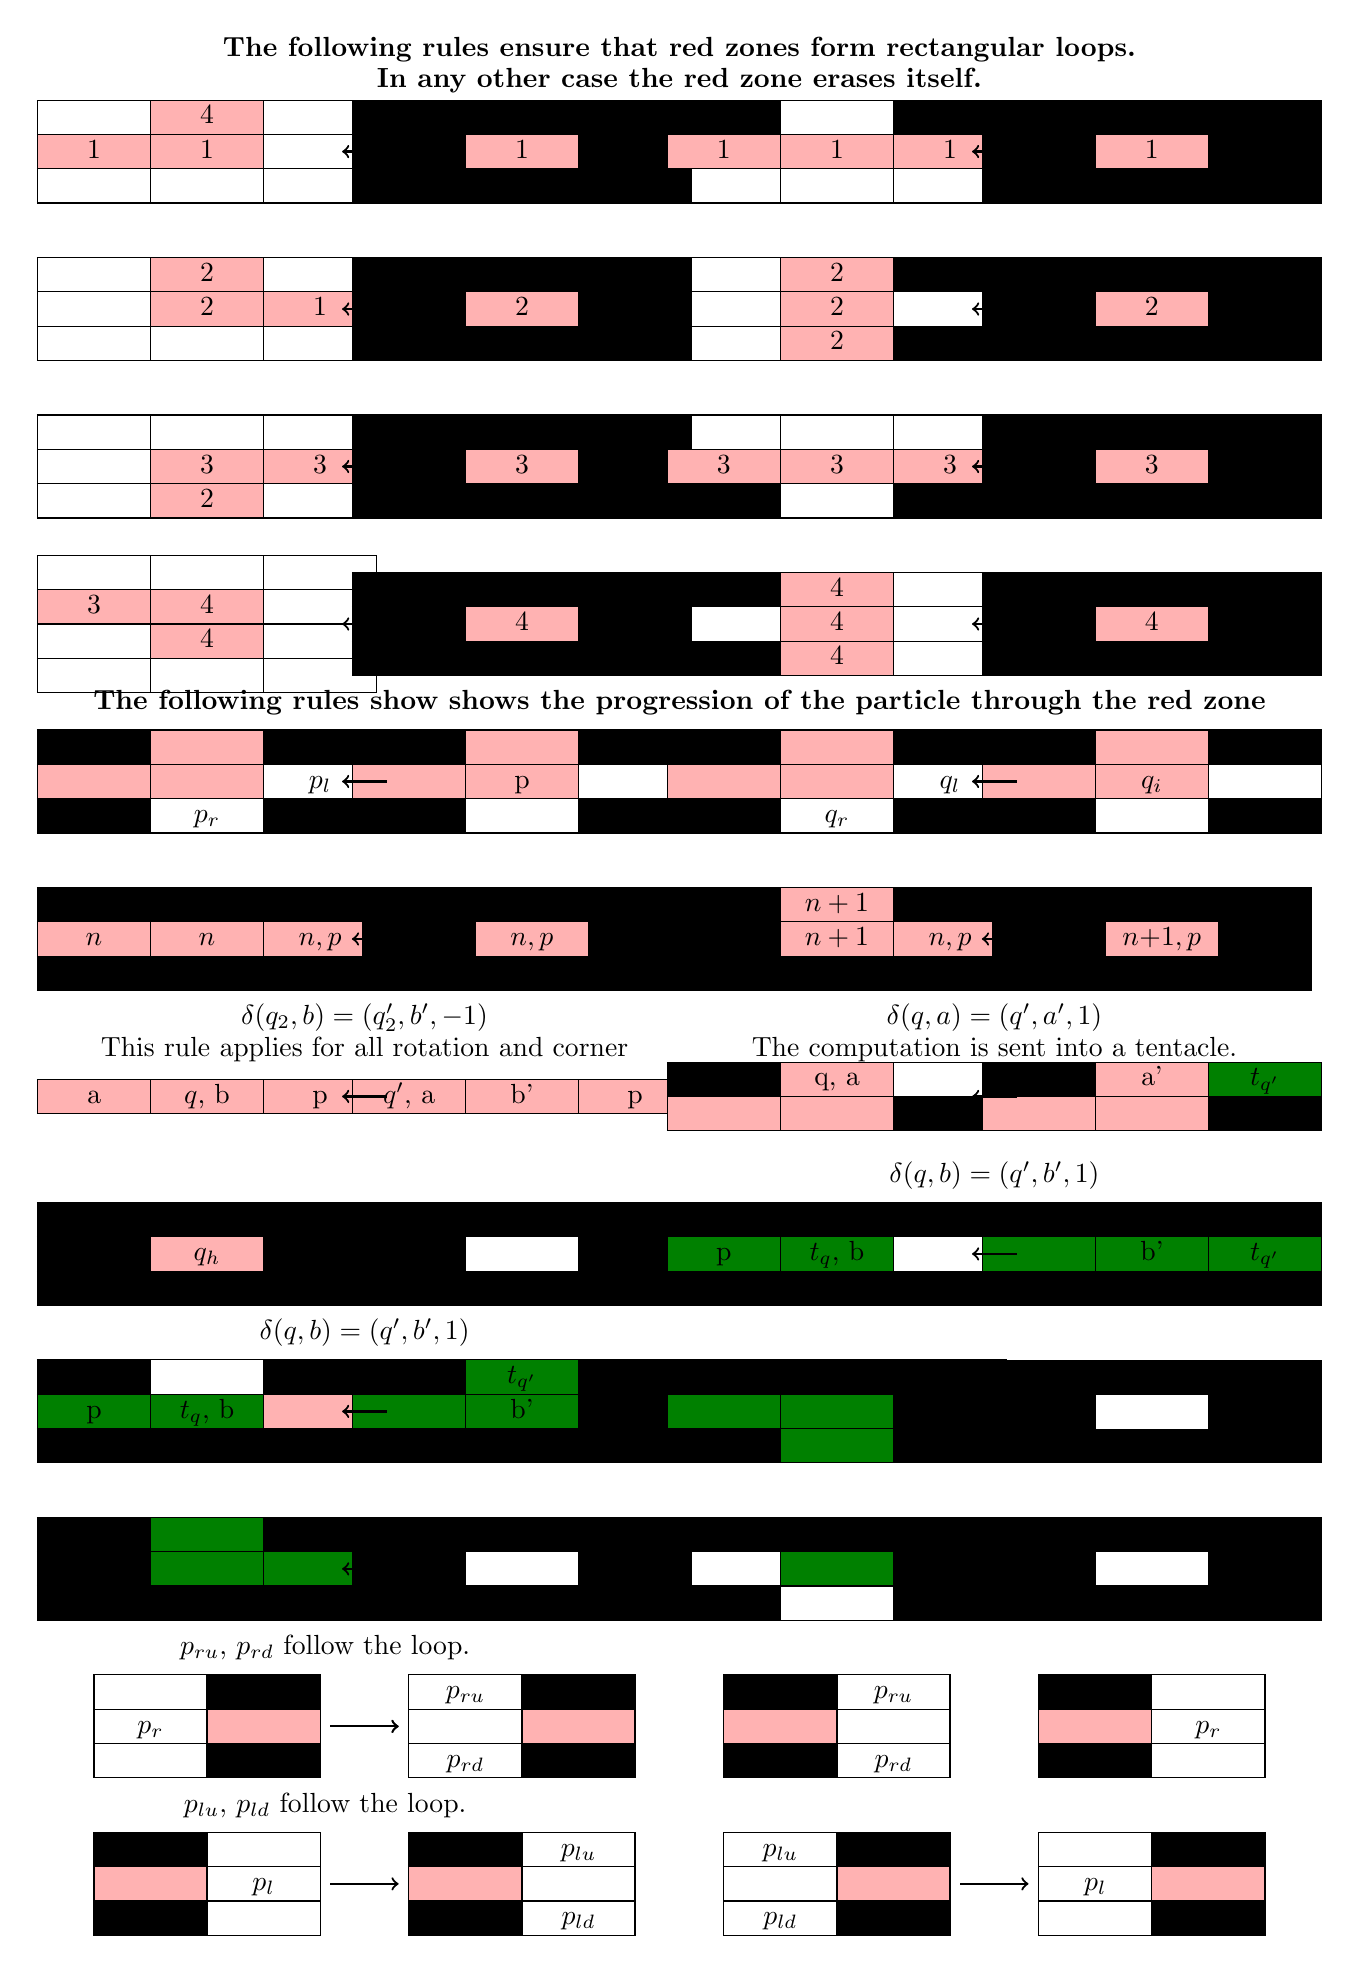
\begin{tikzpicture}

    % règle 1
    \node (tab1) at (0,0) {
        \begin{tabular}{| >{\centering\arraybackslash}m{1cm}| >{\centering\arraybackslash}m{1cm}| >{\centering\arraybackslash}m{1cm}|}
        \hline
         & \cellcolor{red!30}4 &   \\
        \hline
        \cellcolor{red!30}1 & \cellcolor{red!30}1 & \\
        \hline
        & & \\
        \hline
        \end{tabular}
    };

    \node (tab2) at (4, 0){
        \begin{tabular}{| >{\centering\arraybackslash}m{1cm}| >{\centering\arraybackslash}m{1cm}| >{\centering\arraybackslash}m{1cm}|}
        \hline
        \cellcolor{black} & \cellcolor{black} & \cellcolor{black} \\
        \hline
        \cellcolor{black} & \cellcolor{red!30}1 & \cellcolor{black} \\
        \hline
        \cellcolor{black} & \cellcolor{black} & \cellcolor{black} \\
        \hline
        \end{tabular}
    };

    \draw[->, thick] (tab1) -- (tab2);
    %\node at (1.5, 0.7) {};
     \node at (6, 1.3) {\textbf{The following rules ensure that red zones form rectangular loops.}};
     \node at (6, 0.9) {\textbf{In any other case the red zone erases itself.}};
    
    % règle 2
    \node (tab3) at (8,0) {
        \begin{tabular}{| >{\centering\arraybackslash}m{1cm}| >{\centering\arraybackslash}m{1cm}| >{\centering\arraybackslash}m{1cm}|}
        \hline
        \cellcolor{black} & & \cellcolor{black} \\
        \hline
        \cellcolor{red!30}1&\cellcolor{red!30}1&\cellcolor{red!30}1\\
        \hline 
        & & \\
        \hline
        \end{tabular}
    };

    \node (tab4) at (12,0) {
        \begin{tabular}{| >{\centering\arraybackslash}m{1cm}| >{\centering\arraybackslash}m{1cm}| >{\centering\arraybackslash}m{1cm}|}
        \hline
        \cellcolor{black} & \cellcolor{black} & \cellcolor{black} \\
        \hline
        \cellcolor{black} & \cellcolor{red!30}1  & \cellcolor{black} \\
        \hline
        \cellcolor{black} & \cellcolor{black} & \cellcolor{black} \\
        \hline
        \end{tabular}
    };
    \draw[->, thick] (tab3) -- (tab4);
    \node at (7.5, 1) {};

    % règle 3
    \node (tab5) at (0,-2) {
        \begin{tabular}{| >{\centering\arraybackslash}m{1cm}| >{\centering\arraybackslash}m{1cm}| >{\centering\arraybackslash}m{1cm}|}
        \hline
        & \cellcolor{red!30}2 & \\
        \hline
	& \cellcolor{red!30}2 & \cellcolor{red!30}1 \\
        \hline
        & & \\
        \hline
        \end{tabular}
    };

    \node (tab6) at (4,-2) {
        \begin{tabular}{| >{\centering\arraybackslash}m{1cm}| >{\centering\arraybackslash}m{1cm}| >{\centering\arraybackslash}m{1cm}|}
        \hline
	\cellcolor{black} & \cellcolor{black} & \cellcolor{black}\\
        \hline
        \cellcolor{black} & \cellcolor{red!30}2 & \cellcolor{black} \\
        \hline
        \cellcolor{black} & \cellcolor{black} & \cellcolor{black} \\
        \hline
        \end{tabular}
    };
    \draw[->, thick] (tab5) -- (tab6);
    \node at (1.5, -1.2) {};
    
    % règle 4
    \node (tab7) at (8,-2) {
        \begin{tabular}{| >{\centering\arraybackslash}m{1cm}| >{\centering\arraybackslash}m{1cm}| >{\centering\arraybackslash}m{1cm}|}
        \hline
        & \cellcolor{red!30}2 & \cellcolor{black}\\
        \hline
	& \cellcolor{red!30}2 & \\
        \hline
        & \cellcolor{red!30}2 & \cellcolor{black}\\
        \hline
        \end{tabular}
    };

    \node (tab8) at (12, -2){
        \begin{tabular}{| >{\centering\arraybackslash}m{1cm}| >{\centering\arraybackslash}m{1cm}| >{\centering\arraybackslash}m{1cm}|}
        \hline
        \cellcolor{black} & \cellcolor{black} & \cellcolor{black} \\
        \hline
	\cellcolor{black} & \cellcolor{red!30}2 & \cellcolor{black} \\
        \hline
       \cellcolor{black} & \cellcolor{black} & \cellcolor{black} \\
        \hline
        \end{tabular}
    };

    \draw[->, thick] (tab7) -- (tab8);
    \node at (7.5, -1.2) {};
    
    % règle 5
    \node (tab9) at (0,-4) {
        \begin{tabular}{| >{\centering\arraybackslash}m{1cm}| >{\centering\arraybackslash}m{1cm}| >{\centering\arraybackslash}m{1cm}|}
        \hline
        & & \\
        \hline
        & \cellcolor{red!30}3 & \cellcolor{red!30}3 \\
        \hline
	& \cellcolor{red!30}2 &  \\
        \hline
        \end{tabular}
    };

    \node (tab10) at (4,-4) {
       \begin{tabular}{| >{\centering\arraybackslash}m{1cm}| >{\centering\arraybackslash}m{1cm}| >{\centering\arraybackslash}m{1cm}|}
        \hline
        \cellcolor{black} & \cellcolor{black} & \cellcolor{black} \\
        \hline
        \cellcolor{black} & \cellcolor{red!30}3 & \cellcolor{black} \\
        \hline
	\cellcolor{black} &\cellcolor{black} & \cellcolor{black} \\
        \hline
        \end{tabular}
    };
    \draw[->, thick] (tab9) -- (tab10);
    %\node at (1.5, -3.2) {$\delta_e(q, b) = (q', b', 1)$};
    
    % règle 6
    \node (tab11) at (8,-4) {
        \begin{tabular}{| >{\centering\arraybackslash}m{1cm}| >{\centering\arraybackslash}m{1cm}| >{\centering\arraybackslash}m{1cm}|}
        \hline
          & & \\
         \hline
        \cellcolor{red!30}3 & \cellcolor{red!30}3 & \cellcolor{red!30}3\\
        \hline
         \cellcolor{black} & & \cellcolor{black} \\
         \hline
        \end{tabular}
    };

    \node (tab12) at (12, -4){
        \begin{tabular}{| >{\centering\arraybackslash}m{1cm}| >{\centering\arraybackslash}m{1cm}| >{\centering\arraybackslash}m{1cm}|}
        \hline
         \cellcolor{black} & \cellcolor{black} & \cellcolor{black} \\
         \hline
        \cellcolor{black} & \cellcolor{red!30}3 & \cellcolor{black} \\
        \hline
         \cellcolor{black} & \cellcolor{black} & \cellcolor{black} \\
         \hline
        \end{tabular}
    };

    \draw[->, thick] (tab11) -- (tab12);
    %\node at (7.5, -3.2) {$\delta_e(q, b) = (q', b', -1)$};
    
    % règle 7
    \node (tab13) at (0,-6) {
        \begin{tabular}{| >{\centering\arraybackslash}m{1cm}| >{\centering\arraybackslash}m{1cm}| >{\centering\arraybackslash}m{1cm}|}
        \hline
        & &\\
        \hline
        \cellcolor{red!30}3 & \cellcolor{red!30}4 &\\
        \hline
	 & \cellcolor{red!30}4 &  \\
        \hline
        & & \\
        \hline
        \end{tabular}
    };

    \node (tab14) at (4,-6) {
      \begin{tabular}{| >{\centering\arraybackslash}m{1cm}| >{\centering\arraybackslash}m{1cm}| >{\centering\arraybackslash}m{1cm}|}
        \hline
        \cellcolor{black} & \cellcolor{black} & \cellcolor{black} \\
        \hline
        \cellcolor{black} & \cellcolor{red!30}4 & \cellcolor{black}\\
        \hline
	\cellcolor{black} & \cellcolor{black} & \cellcolor{black} \\
        \hline
        \end{tabular}
    };
    \draw[->, thick] (tab13) -- (tab14);
    
    % règle 8
    \node (tab15) at (8,-6) {
        \begin{tabular}{| >{\centering\arraybackslash}m{1cm}| >{\centering\arraybackslash}m{1cm}| >{\centering\arraybackslash}m{1cm}|}
        \hline
	\cellcolor{black} & \cellcolor{red!30}4 &\\
        \hline
        & \cellcolor{red!30}4 &\\
        \hline
        \cellcolor{black}& \cellcolor{red!30}4 & \\
        \hline
        \end{tabular}
    };

    \node (tab16) at (12, -6){
       \begin{tabular}{| >{\centering\arraybackslash}m{1cm}| >{\centering\arraybackslash}m{1cm}| >{\centering\arraybackslash}m{1cm}|}
        \hline
	\cellcolor{black} & \cellcolor{black} & \cellcolor{black} \\
        \hline
        \cellcolor{black} & \cellcolor{red!30}4 & \cellcolor{black} \\
        \hline
        \cellcolor{black} & \cellcolor{black} & \cellcolor{black} \\
        \hline
        \end{tabular}

    };

    \draw[->, thick] (tab15) -- (tab16);
    
    \node at (6, -7) {\textbf{The following rules show shows the progression of the particle through the red zone}};

    
    % règle 9
    \node (tab17) at (0,-8) {
        \begin{tabular}{| >{\centering\arraybackslash}m{1cm}| >{\centering\arraybackslash}m{1cm}| >{\centering\arraybackslash}m{1cm}| >{\centering\arraybackslash}m{1cm}|}
        \hline
        \cellcolor{black} & \cellcolor{red!30} & $\cellcolor{black}$\\
        \hline
	\cellcolor{red!30} & \cellcolor{red!30} & $p_l$ \\
        \hline
        \cellcolor{black} & $p_r$ & \cellcolor{black}\\
        \hline
        \end{tabular}
    };

    \node (tab18) at (4,-8) {
         \begin{tabular}{| >{\centering\arraybackslash}m{1cm}| >{\centering\arraybackslash}m{1cm}| >{\centering\arraybackslash}m{1cm}| >{\centering\arraybackslash}m{1cm}|}
        \hline
        \cellcolor{black} & \cellcolor{red!30} & $\cellcolor{black}$\\
        \hline
	\cellcolor{red!30} & \cellcolor{red!30}p & \\
        \hline
        \cellcolor{black} &  & \cellcolor{black}\\
        \hline
        \end{tabular}
     };
    \draw[->, thick] (tab17) -- (tab18);
    %\node at (1.5, -3.2) {$\delta_e(q, b) = (q', b', 1)$};
    
    % règle 10
    \node (tab19) at (8,-8) {
        \begin{tabular}{| >{\centering\arraybackslash}m{1cm}| >{\centering\arraybackslash}m{1cm}| >{\centering\arraybackslash}m{1cm}| >{\centering\arraybackslash}m{1cm}|}
        \hline
        \cellcolor{black} & \cellcolor{red!30} & $\cellcolor{black}$\\
        \hline
	\cellcolor{red!30} & \cellcolor{red!30} & $q_l$ \\
        \hline
        \cellcolor{black} & $q_r$ & \cellcolor{black}\\
        \hline
        \end{tabular}
    };

    \node (tab20) at (12, -8){
        \begin{tabular}{| >{\centering\arraybackslash}m{1cm}| >{\centering\arraybackslash}m{1cm}| >{\centering\arraybackslash}m{1cm}| >{\centering\arraybackslash}m{1cm}|}
        \hline
        \cellcolor{black} & \cellcolor{red!30} & $\cellcolor{black}$\\
        \hline
	\cellcolor{red!30} & \cellcolor{red!30}$q_i$ &  \\
        \hline
        \cellcolor{black} & & \cellcolor{black}\\
        \hline
        \end{tabular}
    };

    \draw[->, thick] (tab19) -- (tab20);
    
     % règle 11
    \node (tab21) at (0,-10) {
        \begin{tabular}{| >{\centering\arraybackslash}m{1cm}| >{\centering\arraybackslash}m{1cm}| >{\centering\arraybackslash}m{1cm}|}
        \hline
        \cellcolor{black} & \cellcolor{black} & \cellcolor{black} \\
        \hline
        \cellcolor{red!30}$n$ & \cellcolor{red!30}$n$ & \cellcolor{red!30}$n, p$ \\
        \hline
        \cellcolor{black} & \cellcolor{black} & \cellcolor{black} \\
        \hline
        \end{tabular}
    };

    \node (tab22) at (4,-10) {
       \begin{tabular}{| >{\centering\arraybackslash}m{1cm}| >{\centering\arraybackslash}m{1cm}|>{\centering\arraybackslash}m{0.75cm}|}
        \hline
        \cellcolor{black} & \cellcolor{black} & \cellcolor{black} \\
        \hline
        \cellcolor{black} & \cellcolor{red!30}$n, p$ & \cellcolor{black} \\
        \hline
        \cellcolor{black} & \cellcolor{black} & \cellcolor{black} \\
        \hline
        \end{tabular}
    };
    \draw[->, thick] (tab21) -- (tab22);
    %\node at (1.5, -9.4) {Particle p is guided by $1$, $2$, $3$, $4$.};
    
    % règle 12
    \node (tab23) at (8,-10) {
        \begin{tabular}{| >{\centering\arraybackslash}m{1cm}| >{\centering\arraybackslash}m{1cm}| >{\centering\arraybackslash}m{1cm}|}
        \hline
         \cellcolor{black} & \cellcolor{red!30}$n+1$ & \cellcolor{black} \\
         \hline
        \cellcolor{black} & \cellcolor{red!30}$n+1$ & \cellcolor{red!30}$n, p$ \\
        \hline
         \cellcolor{black} & \cellcolor{black} & \cellcolor{black} \\
         \hline
        \end{tabular}
    };

    \node (tab24) at (12, -10){
        \begin{tabular}{| >{\centering\arraybackslash}m{1cm}| >{\centering\arraybackslash}m{1cm}|>{\centering\arraybackslash}m{0.75cm}|}
        \hline
         \cellcolor{black} & \cellcolor{black} & \cellcolor{black} \\
         \hline
        \cellcolor{black} & \cellcolor{red!30}$n+1, p$ & \cellcolor{black}\\
        \hline
         \cellcolor{black} & \cellcolor{black} & \cellcolor{black} \\
         \hline
        \end{tabular}
    };

    \draw[->, thick] (tab23) -- (tab24);
     %\node at (7.5, -9.4) {Erase the loop.};
    
     % règle 13
    \node (tab25) at (0,-12) {
        \begin{tabular}{| >{\centering\arraybackslash}m{1cm}| >{\centering\arraybackslash}m{1cm}| >{\centering\arraybackslash}m{1cm}|}
        \hline
        \cellcolor{red!30}a & \cellcolor{red!30}$q$, b & \cellcolor{red!30}p \\
        \hline
        \end{tabular}
    };

    \node (tab26) at (4,-12) {
        \begin{tabular}{| >{\centering\arraybackslash}m{1cm}| >{\centering\arraybackslash}m{1cm}| >{\centering\arraybackslash}m{1cm}|}
        \hline
        \cellcolor{red!30}$q'$, a & \cellcolor{red!30}b' & \cellcolor{red!30}p \\
        \hline
        \end{tabular}
    };
    \draw[->, thick] (tab25) -- (tab26);
    \node at (2, -11) {$\delta(q_2, b) = (q_2', b', -1)$};
    \node at (2, -11.4) {This rule applies for all rotation and corner};
    
    % règle 14
    \node (tab27) at (8,-12) {
        \begin{tabular}{| >{\centering\arraybackslash}m{1cm}| >{\centering\arraybackslash}m{1cm}| >{\centering\arraybackslash}m{1cm}|}
        \hline
        \cellcolor{black} & \cellcolor{red!30}q, a &  \\
        \hline
	\cellcolor{red!30} & \cellcolor{red!30} & \cellcolor{black}  \\
        \hline 
        \end{tabular}
    };

    \node (tab28) at (12, -12){
       \begin{tabular}{| >{\centering\arraybackslash}m{1cm}| >{\centering\arraybackslash}m{1cm}| >{\centering\arraybackslash}m{1cm}|}
        \hline
        \cellcolor{black} & \cellcolor{red!30}a' & \cellcolor{green!50!black}$t_{q'}$  \\
        \hline
	\cellcolor{red!30} & \cellcolor{red!30} & \cellcolor{black} \\
        \hline 
        \end{tabular}
    };

    \draw[->, thick] (tab27) -- (tab28);
    \node at (10, -11) {$\delta(q, a) = (q', a', 1)$};
    \node at (10, -11.4) {The computation is sent into a tentacle.};
    
    % règle 15
    \node (tab29) at (0,-14) {
        \begin{tabular}{| >{\centering\arraybackslash}m{1cm}| >{\centering\arraybackslash}m{1cm}| >{\centering\arraybackslash}m{1cm}|}
        \hline
        \cellcolor{black} & \cellcolor{black} & \cellcolor{black} \\
        \hline
        \cellcolor{black} & \cellcolor{red!30}$q_h$ &\cellcolor{black} \\
        \hline
        \cellcolor{black} & \cellcolor{black} & \cellcolor{black} \\
        \hline
        \end{tabular}
    };

    \node (tab30) at (4,-14) {
         \begin{tabular}{| >{\centering\arraybackslash}m{1cm}| >{\centering\arraybackslash}m{1cm}| >{\centering\arraybackslash}m{1cm}|}
        \hline
        \cellcolor{black} & \cellcolor{black} & \cellcolor{black} \\
        \hline
        \cellcolor{black} &  &\cellcolor{black} \\
        \hline
        \cellcolor{black} & \cellcolor{black} & \cellcolor{black} \\
        \hline
        \end{tabular}
    };
    \draw[->, thick] (tab29) -- (tab30);
    %\node at (1.5, -13.4) {Erase the loop.};
    
    % règle 16
    \node (tab31) at (8,-14) {
        \begin{tabular}{| >{\centering\arraybackslash}m{1cm}| >{\centering\arraybackslash}m{1cm}| >{\centering\arraybackslash}m{1cm}|}
        \hline
        \cellcolor{black} & \cellcolor{black} & \cellcolor{black} \\
        \hline
        \cellcolor{green!50!black}p & \cellcolor{green!50!black}$t_q$, b &  \\
        \hline
        \cellcolor{black} & \cellcolor{black} & \cellcolor{black} \\
        \hline
        \end{tabular}
    };

    \node (tab32) at (12, -14){
        \begin{tabular}{| >{\centering\arraybackslash}m{1cm}| >{\centering\arraybackslash}m{1cm}| >{\centering\arraybackslash}m{1cm}|}
        \hline
        \cellcolor{black} & \cellcolor{black} & \cellcolor{black} \\
        \hline
        \cellcolor{green!50!black} & \cellcolor{green!50!black} b' & \cellcolor{green!50!black}$t_{q'}$ \\
        \hline
        \cellcolor{black} & \cellcolor{black} & \cellcolor{black} \\
        \hline
        \end{tabular}
    };

    \draw[->, thick] (tab31) -- (tab32);
    \node at (10, -13) {$\delta(q, b) = (q', b', 1)$};
    
    % règle 17
    \node (tab33) at (0,-16) {
        \begin{tabular}{| >{\centering\arraybackslash}m{1cm}| >{\centering\arraybackslash}m{1cm}| >{\centering\arraybackslash}m{1cm}|}
        \hline
        \cellcolor{black} &  & \cellcolor{black} \\
        \hline
        \cellcolor{green!50!black}p & \cellcolor{green!50!black}$t_q$, b & \cellcolor{red!30} \\
        \hline
        \cellcolor{black} & \cellcolor{black} & \cellcolor{black} \\
        \hline
        \end{tabular}
    };

    \node (tab34) at (4,-16) {
        \begin{tabular}{| >{\centering\arraybackslash}m{1cm}| >{\centering\arraybackslash}m{1cm}| >{\centering\arraybackslash}m{1cm}|}
        \hline
        \cellcolor{black} & \cellcolor{green!50!black}$t_{q'}$ & \cellcolor{black} \\
        \hline
        \cellcolor{green!50!black} & \cellcolor{green!50!black}b' & \cellcolor{black} \\
        \hline
        \cellcolor{black} & \cellcolor{black} & \cellcolor{black} \\
        \hline
        \end{tabular}
    };
   \draw[->, thick] (tab33) -- (tab34);
   \node at (2, -15) {$\delta(q, b) = (q', b', 1)$};
    
    % règle 18
    \node (tab35) at (8,-16) {
       \begin{tabular}{| >{\centering\arraybackslash}m{1cm}| >{\centering\arraybackslash}m{1cm}|>{\centering\arraybackslash}m{1cm}|}
        \hline
        \cellcolor{black} & \cellcolor{black} & \cellcolor{black} \\
        \hline
        \cellcolor{green!50!black} & \cellcolor{green!50!black} & \cellcolor{black} \\
	\hline
	\cellcolor{black} & \cellcolor{green!50!black} & \cellcolor{black} \\
	\hline
        \end{tabular}
    };

    \node (tab36) at (12, -16){
         \begin{tabular}{| >{\centering\arraybackslash}m{1cm}| >{\centering\arraybackslash}m{1cm}|>{\centering\arraybackslash}m{1cm}|}
        \hline
         \cellcolor{black} & \cellcolor{black} & \cellcolor{black} \\
         \hline
        \cellcolor{black} & & \cellcolor{black} \\
	\hline
	\cellcolor{black} & \cellcolor{black}  & \cellcolor{black}\\
        \end{tabular}
    };

    \draw[->, thick] (tab35) -- (tab36);
    %\node at (7.5, -15) {x check that the tentacle is linked };
    %\node at (7.5, -15.4) {to a turing machine, erase otherwise.};

    
    % règle 19
    \node (tab33) at (0,-18) {
        \begin{tabular}{| >{\centering\arraybackslash}m{1cm}| >{\centering\arraybackslash}m{1cm}| >{\centering\arraybackslash}m{1cm}|}
        \hline
        \cellcolor{black} & \cellcolor{green!50!black} & \cellcolor{black}  \\
	\hline
	\cellcolor{black} & \cellcolor{green!50!black} & \cellcolor{green!50!black} \\
	\hline
	 \cellcolor{black} & \cellcolor{black} & \cellcolor{black}\\
	\hline
        \end{tabular}

    };

    \node (tab34) at (4,-18) {
         \begin{tabular}{| >{\centering\arraybackslash}m{1cm}| >{\centering\arraybackslash}m{1cm}| >{\centering\arraybackslash}m{1cm}|}
        \hline
        \cellcolor{black} & \cellcolor{black} & \cellcolor{black}  \\
	\hline
	\cellcolor{black} &  & \cellcolor{black} \\
	\hline
	 \cellcolor{black} & \cellcolor{black} & \cellcolor{black}\\
	\hline
	\end{tabular}

    };
    \draw[->, thick] (tab33) -- (tab34);
    
    % règle 20
    \node (tab35) at (8,-18) {
       \begin{tabular}{| >{\centering\arraybackslash}m{1cm}| >{\centering\arraybackslash}m{1cm}| >{\centering\arraybackslash}m{1cm}|}
        \hline
        \cellcolor{black} & \cellcolor{black} & \cellcolor{black}  \\
	\hline
	& \cellcolor{green!50!black} & \cellcolor{black} \\
	\hline
	 \cellcolor{black} & & \cellcolor{black}\\
	\hline
        \end{tabular}
    };

    \node (tab36) at (12, -18){
         \begin{tabular}{| >{\centering\arraybackslash}m{1cm}| >{\centering\arraybackslash}m{1cm}| >{\centering\arraybackslash}m{1cm}|}
        \hline
        \cellcolor{black} & \cellcolor{black} & \cellcolor{black}  \\
	\hline
	\cellcolor{black} &  & \cellcolor{black} \\
	\hline
	 \cellcolor{black} & \cellcolor{black} & \cellcolor{black}\\
	\hline
	\end{tabular}
    };

    \draw[->, thick] (tab35) -- (tab36);
    
    % règle 21
    \node (tab37) at (0,-20) {
        \begin{tabular}{| >{\centering\arraybackslash}m{1cm}| >{\centering\arraybackslash}m{1cm}| >{\centering\arraybackslash}m{1cm}|}
        \hline
        & \cellcolor{black}\\
        \hline
        $p_r$ & \cellcolor{red!30} \\
        \hline
	 & \cellcolor{black} \\
        \hline
        \end{tabular}
    };

    \node (tab38) at (4, -20){
        \begin{tabular}{| >{\centering\arraybackslash}m{1cm}| >{\centering\arraybackslash}m{1cm}|}
        \hline
        $p_{ru}$ & \cellcolor{black} \\
        \hline
	 & \cellcolor{red!30}  \\
        \hline
        $p_{rd}$ & \cellcolor{black}\\
        \hline
        \end{tabular}
    };

    \draw[->, thick] (tab37) -- (tab38);
    \node at (1.5, -19) {$p_{ru}$, $p_{rd}$ follow the loop.};

    
      % règle 22
    \node (tab39) at (8,-20) {
        \begin{tabular}{| >{\centering\arraybackslash}m{1cm}| >{\centering\arraybackslash}m{1cm}|}
        \hline
        \cellcolor{black} & $p_{ru}$\\
        \hline
	\cellcolor{red!30}  & \\
        \hline
        \cellcolor{black} & $p_{rd}$\\
        \hline
        \end{tabular}
    };

    \node (tab40) at (12, -20){
        \begin{tabular}{| >{\centering\arraybackslash}m{1cm}| >{\centering\arraybackslash}m{1cm}|}
        \hline
        \cellcolor{black} & \\
        \hline
	\cellcolor{red!30}  & $p_r$\\
        \hline
        \cellcolor{black} & \\
        \hline
        \end{tabular}
    };

    \draw[->, thick] (tab37) -- (tab38);

% règle 23
    \node (tab39) at (0,-22) {
        \begin{tabular}{| >{\centering\arraybackslash}m{1cm}| >{\centering\arraybackslash}m{1cm}| >{\centering\arraybackslash}m{1cm}|}
        \hline
        \cellcolor{black} & \\
        \hline
        \cellcolor{red!30} & $p_l$\\
        \hline
	\cellcolor{black} & \\
        \hline
        \end{tabular}
    };

    \node (tab40) at (4, -22){
        \begin{tabular}{| >{\centering\arraybackslash}m{1cm}| >{\centering\arraybackslash}m{1cm}|}
        \hline
        \cellcolor{black} & $p_{lu}$ \\
        \hline
	 \cellcolor{red!30}  & \\
        \hline
        \cellcolor{black} & $p_{ld}$\\
        \hline
        \end{tabular}
    };

    \draw[->, thick] (tab39) -- (tab40);
    \node at (1.5, -21) {$p_{lu}$, $p_{ld}$ follow the loop.};

    
      % règle 24
    \node (tab41) at (8,-22) {
        \begin{tabular}{| >{\centering\arraybackslash}m{1cm}| >{\centering\arraybackslash}m{1cm}|}
        \hline
        $p_{lu}$ & \cellcolor{black} \\
        \hline
	& \cellcolor{red!30} \\
        \hline
        $p_{ld}$ & \cellcolor{black} \\
        \hline
        \end{tabular}
    };

    \node (tab42) at (12, -22){
        \begin{tabular}{| >{\centering\arraybackslash}m{1cm}| >{\centering\arraybackslash}m{1cm}|}
        \hline
        & \cellcolor{black} \\
        \hline
	$p_l$ & \cellcolor{red!30} \\
        \hline
        & \cellcolor{black} \\
        \hline
        \end{tabular}
    };

    \draw[->, thick] (tab41) -- (tab42);





\end{tikzpicture}}
\end{center}
\caption{Main rules for the transition function of the 2 dimensional cellular automaton $G_e$. Black cells act as wildcards and can match any state in the neighborhood.}
\label{fig:transition2D}
\end{figure*}
